\documentclass[../informe2.tex]{subfiles}
\begin{document}

Que fue lo que se logró con la experimentación, incluir tablas y parámetros,
gráficos, etc. lo más explicativo posible. Además destacar puntos
importantes del problema, características de las instancias que influyeron
en los resultados, valores de parámetros que influyeron en los resultados,
análisis de calidad de las soluciones encontradas a través del tiempo,
análisis en profundidad de la técnica vs los resultados obtenidos,
valores promedio, desviaciones, \textbf{comparaciones con resultados
	de la literatura}, etc. También debería discutir qué cosas podría
haber agregado o quedan como desafíos para trabajo futuro en su algoritmo.

% Please add the following required packages to your document preamble:
% \usepackage{booktabs}
\begin{table}[h]
	\small
	\centering
	\begin{tabular}{@{}lrrrrrrrrrr@{}}
		\toprule
		Estadística/Instancia                       & a1\_1 & a1\_2 & a1\_3 & a1\_4 & a1\_5 & a2\_1  & a2\_2 & a2\_3 & a2\_4 & a2\_5 \\ \midrule
		Total de servicios                          & 79    & 980   & 216   & 142   & 981   & 1000   & 170   & 129   & 180   & 153   \\
		\begin{tabular}[c]{@{}l@{}}Servicios sin dependencias\\ y spreadmin nulo\end{tabular} & 73    & 970   & 116   & 44    & 972   & 1000   & 92    & 4     & 55    & 29    \\
		\%                                          & 92.41 & 98.98 & 53.70 & 30.99 & 99.08 & 100.00 & 54.12 & 3.10  & 30.56 & 18.95 \\ \bottomrule
	\end{tabular}
	
	\bigskip
	
	\begin{tabular}{@{}lrrrrrrrrrr@{}}
		\toprule
		Estadística/Instancia                                                                 & b\_1  & b\_2  & b\_3  & b\_4  & b\_5  & b\_6  & b\_7  & b\_8  & b\_9  & b\_10 \\ \midrule
		Total de servicios                                                                    & 2512  & 2462  & 15025 & 1732  & 35082 & 14680 & 15050 & 45030 & 4609  & 4896  \\
		\begin{tabular}[c]{@{}l@{}}Servicios sin dependencias\\ y spreadmin nulo\end{tabular} & 2012  & 1962  & 14025 & 732   & 34082 & 13680 & 14050 & 44030 & 3609  & 3896  \\
		\%                                                                                    & 80.10 & 79.69 & 93.34 & 42.26 & 97.15 & 93.19 & 93.36 & 97.78 & 78.30 & 79.58 \\ \bottomrule
	\end{tabular}
	\caption{\small Por cada instancia, se determina la cantidad de servicios que no poseen dependencias y tienen un mínimo de dispersión igual a cero.}
	\label{tabla:analisis-servicios}
\end{table}

\begin{figure}[ht]
	\centering
	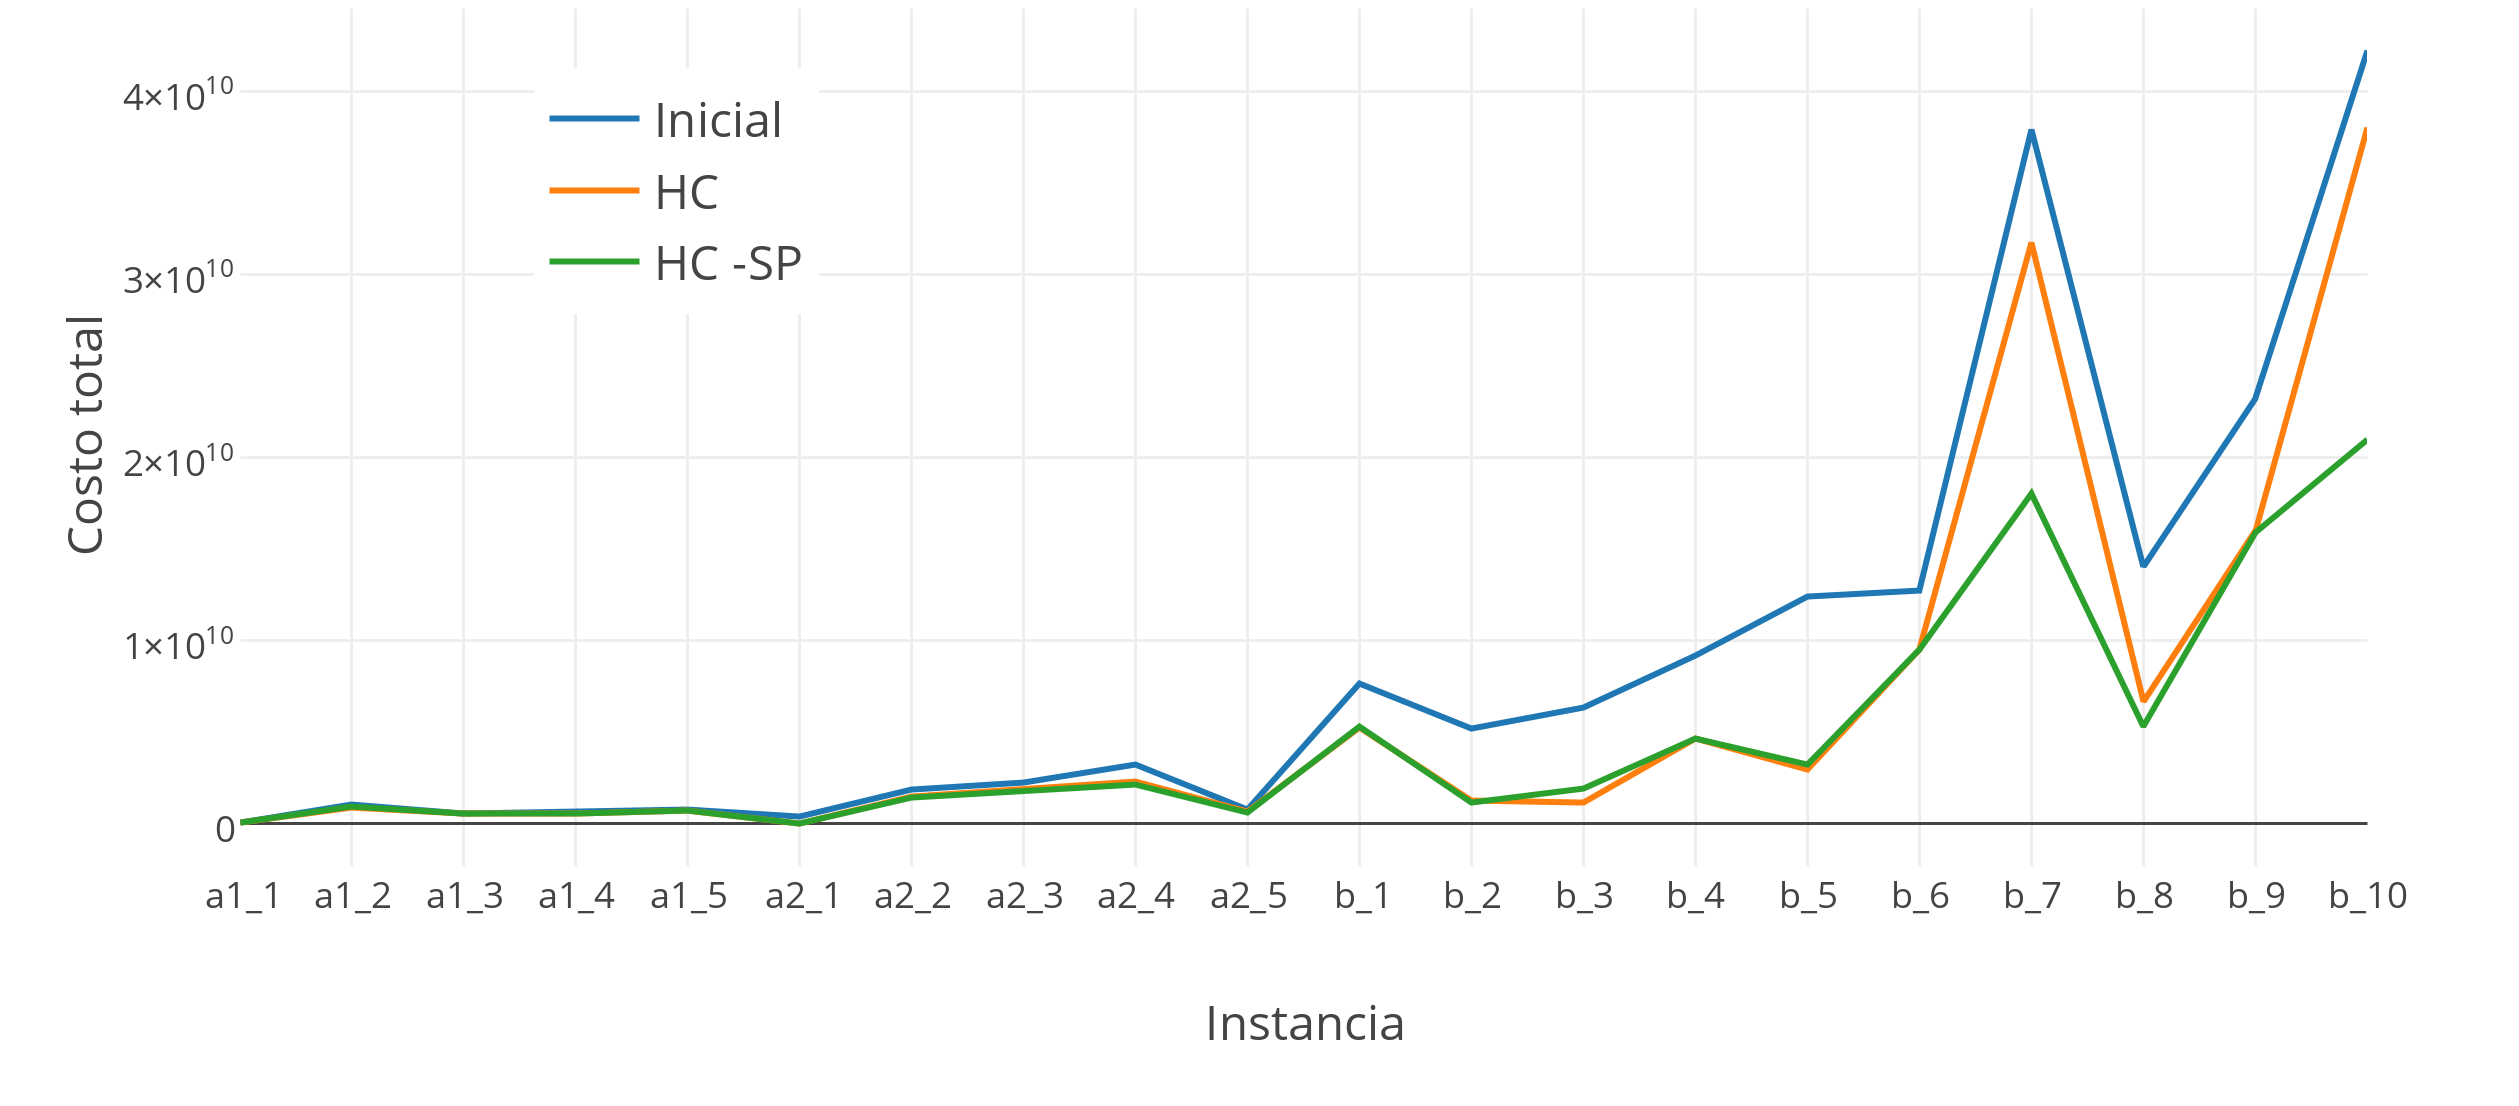
\includegraphics[width=0.45\textwidth]{comparativa-hc.png}
	\caption{\small}
	\label{fig:comparativa-hc}
\end{figure}

\begin{figure}[ht]
	\centering
	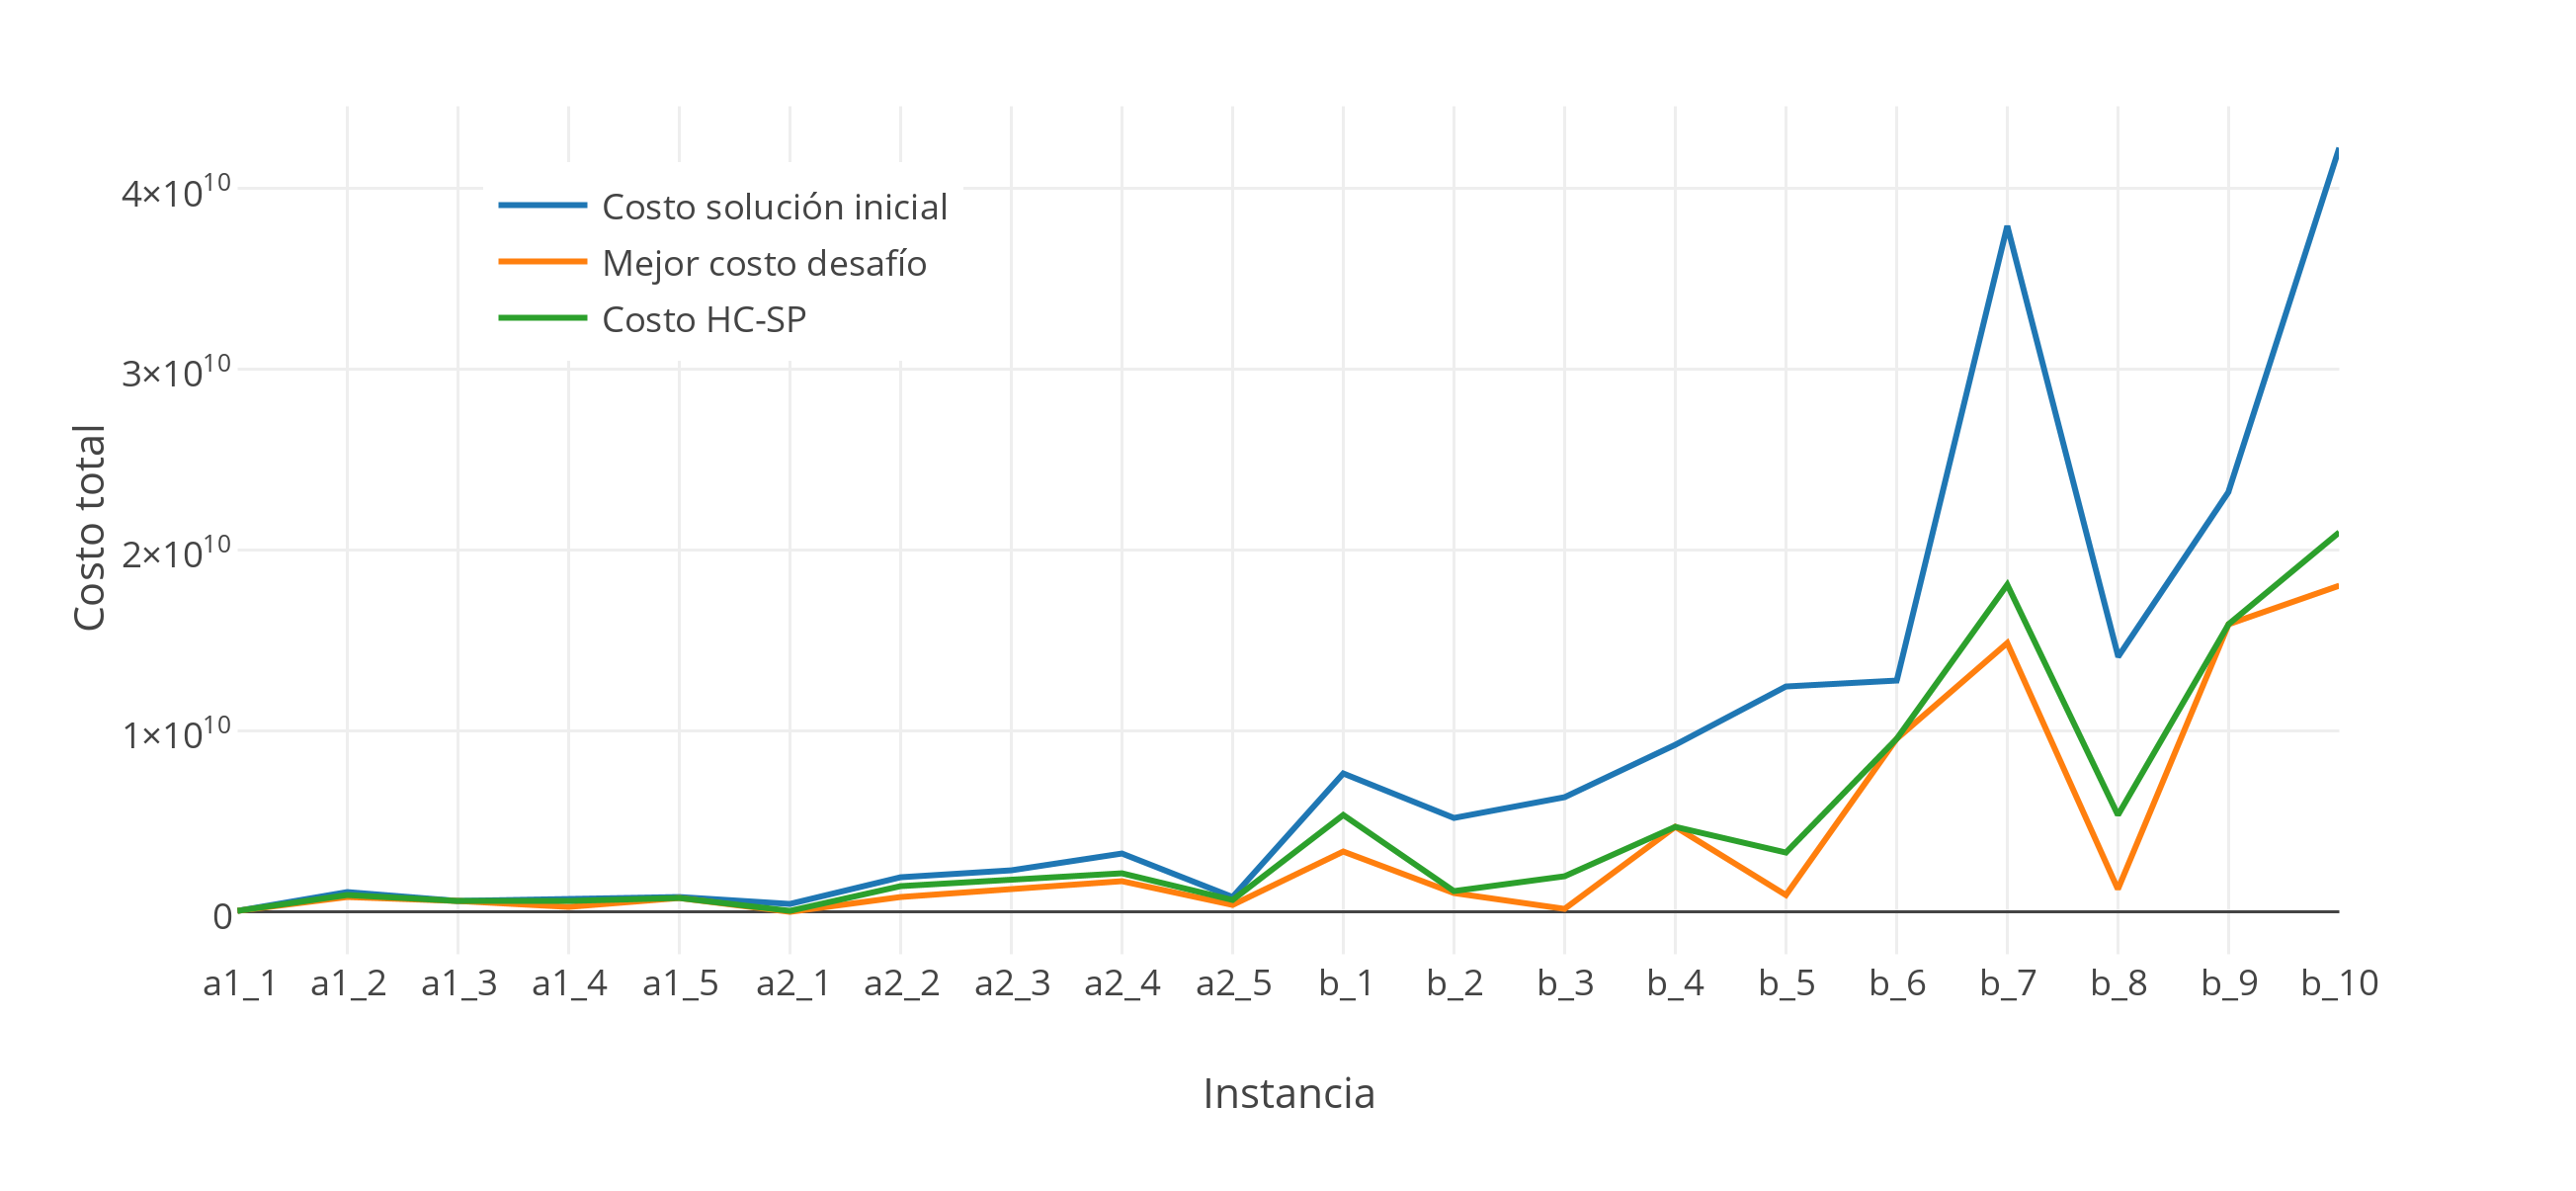
\includegraphics[width=0.45\textwidth]{comparativa-hc-best-challenge.png}
	\caption{\small}
	\label{fig:comparativa-hc-best-challenge}
\end{figure}


\end{document}

